\usetikzlibrary{arrows}
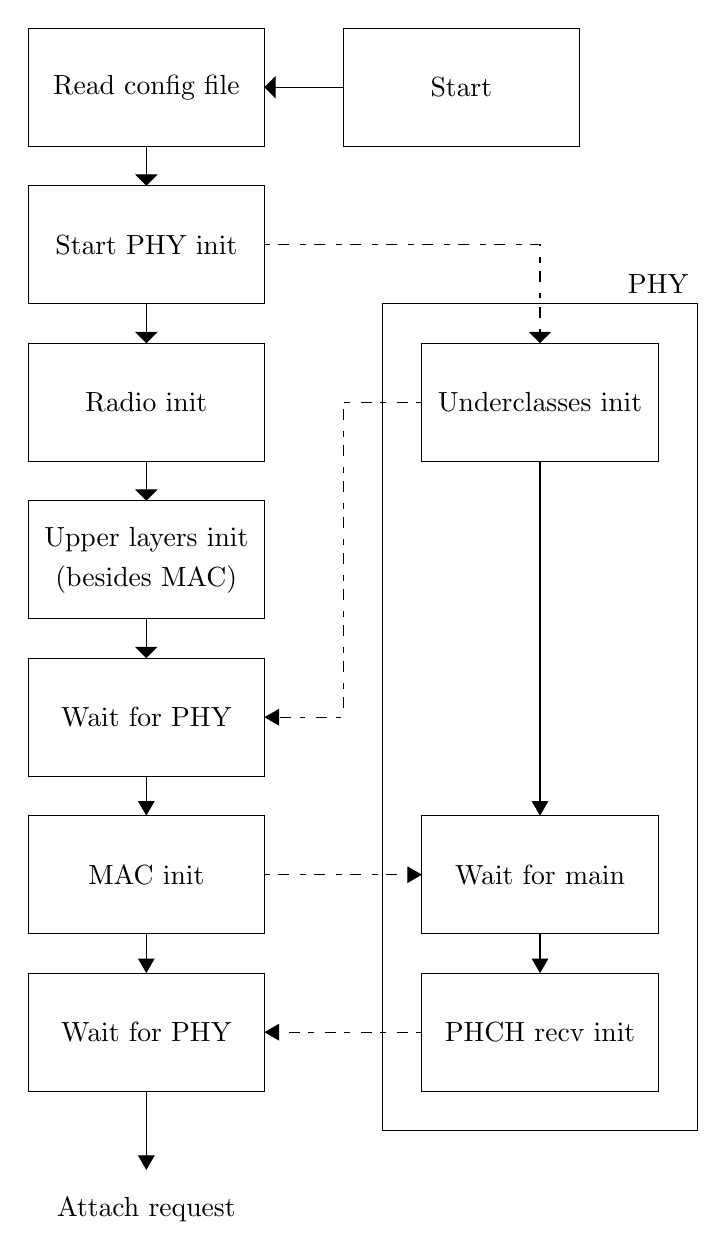
\begin{tikzpicture}


\draw  (-4,3) rectangle (-1,1.5);
\draw  (-8,3) rectangle (-5,1.5);
\draw  (-8,1) rectangle (-5,-0.5);
\draw  (-8,-1) rectangle (-5,-2.5);
\draw  (-8,-3) rectangle (-5,-4.5);
\draw  (-3,-1) rectangle (0,-2.5);
\draw  (-3,-9) rectangle (0,-10.5);
\draw  (-8,-5) rectangle (-5,-6.5);
\draw  (-3.5,-0.5) rectangle (0.5,-11);

\draw [-triangle 90](-4,2.25) -- (-5,2.25);
\draw [-triangle 90](-6.5,1.5) -- (-6.5,1);
\draw [-triangle 90](-6.5,-0.5) -- (-6.5,-1);
\draw [-triangle 90](-6.5,-2.5) -- (-6.5,-3);
\draw [-triangle 90](-6.5,-4.5) -- (-6.5,-5);
\draw [dash pattern=on 2pt off 3pt on 4pt off 4pt][-triangle 90](-5,0.25) -- (-1.5,0.25) -- (-1.5,-1);


\node at (-2.5,2.25) {Start};
\node at (-6.5,2.25) {Read config file};
\node at (-6.5,0.25) {Start PHY init};
\node at (-6.5,-1.75) {Radio init};
\node at (-6.5,-3.5) {Upper layers init};
\node at (-6.5,-5.75) {Wait for PHY};
\node at (-1.5,-1.75) {Underclasses init};
\node at (-1.5,-9.75) {PHCH recv init};


\node at (0,-0.25) {PHY};
\node at (-6.5,-4) {(besides MAC)};

\draw [-triangle 60](-6.5,-6.5) -- (-6.5,-7);
\draw  (-8,-7) rectangle (-5,-8.5);
\draw  (-8,-9) rectangle (-5,-10.5);
\draw [-triangle 60](-6.5,-8.5) -- (-6.5,-9);
\node at (-6.5,-7.75) {MAC init};
\node at (-6.5,-9.75) {Wait for PHY};
\draw [-triangle 60](-6.5,-10.5) -- (-6.5,-11.5);
\node at (-6.5,-12) {Attach request};
\draw [-triangle 60] (-3,-7) rectangle (0,-8.5);
\draw [-triangle 60](-1.5,-2.5) -- (-1.5,-7);
\draw [-triangle 60](-1.5,-8.5) -- (-1.5,-9);
\node at (-1.5,-7.75) {Wait for main};
\draw [dash pattern=on 2pt off 3pt on 4pt off 4pt][-triangle 60](-3,-1.75) -- (-4,-1.75) -- (-4,-5.75) -- (-5,-5.75);
\draw [dash pattern=on 2pt off 3pt on 4pt off 4pt][-triangle 60](-5,-7.75) -- (-3,-7.75);
\draw [dash pattern=on 2pt off 3pt on 4pt off 4pt][-triangle 60](-3,-9.75) -- (-5,-9.75);
\end{tikzpicture}